\ifx\wholebook\relax \else

\documentclass[b5paper]{ctexart}
\usepackage[nomarginpar
  %, margin=.5in
]{geometry}

\addtolength{\oddsidemargin}{-0.05in}
\addtolength{\evensidemargin}{-0.05in}
\addtolength{\textwidth}{0.1in}

\usepackage[cn]{../prelude}

\setcounter{page}{1}

\begin{document}

\title{复数}

\author{刘新宇
\thanks{{\bfseries 刘新宇} \newline
  Email: liuxinyu99@hotmail.com \newline}
  }

\maketitle
\fi

\markboth{复数}{数的旅程}

\ifx\wholebook\relax
\chapter{复数}
\fi

%% On earth there is nothing great but man; and in man there is nothing great but mind.
\epigraph{地球上最伟大的是人,人之中最伟大的是心灵}{威廉·汉密尔顿}

读过金庸武侠小说的读者一定对“华山论剑”津津乐道。天下武林中的顶级高手约定在华山比武论剑。大家各自身怀秘不外传的绝世武功,通过比武确定谁是真正的天下武功第一。十六世纪的意大利也上演了精彩的华山论剑。只不过没有刀光剑影、没有拳脚身法,而是一场关于数学与荣誉的挑战。1535年2月13日深夜,塔尔塔利亚在威尼斯的家中踱来踱去,为即将到来的挑战苦思冥想。文艺复兴时期的意大利,学着间经常进行骑士般的公开挑战。这种挑战并不使用刀剑或者火枪进行决斗,双方各自向对方提出同等数目的数学题目,并在规定的时间内作答。正确答出多的人获胜。胜利的一方赢得荣誉或一定数目的奖金。这种一对一的“单挑”发生在知名学者之间,通常在大教堂这类城市公共场所进行,引起众人的围观。有时甚至市长或者贵族也会前来观看,因而使得胜负具有非常的意义,影响双方的社会地位、学术评价甚至职业发展。

例如1225年,神圣罗马帝国皇帝腓特烈二世在西西里行宫接见了斐波那契。宫廷学者看不起商人出身的数学家,于是向斐波那契发起了挑战。斐波那契成功解决了全部问题,为自己赢得了荣誉。这些题目中包含了一道一元三次方程\footnote{当时还没有代数符号,是用文字描述的,如:找到一个数,其立方加上其平方的两倍再加上其十倍是二十。}:\[x^3 + 2x^2 + 10x = 20\]

斐波那契使用古巴比伦的60进制数值解法给出了正确答案:
\[
1^022^{I}7^{II}42^{III}33^{IV}4^{V}40^{VI} = 1 + \frac{22}{60} + \frac{7}{60^2} + \frac{42}{60^3} + \dotsb
\]

相当于十进制小数1.3688081075,精确到了小数点后9位。这种公开挑战也造成了一种奇特现象:学者们把自己的研究成果视为高度机密。因为这样可以使得他在与别人的挑战中获得优势。一旦泄露,对方就能解出自己提出的问题。学者们在生前不发表自己的成果,而是在死前传给自己信任的门生。这在“不发表就发霉”的今天是很难理解的\cite{HanXueTao2012}。

塔尔塔利亚面临的挑战就是关于三次方程的,对手名叫费奥尔\footnote{安东尼奥・马里亚・费奥尔,Antonio Maria Fior}。尽管古巴比伦人在公元前2000左右就掌握了一元二次方程的解法,但人们在接下来的4000多年一直没有突破一般三次方程的解法。人们并不满足于斐波那契的数值解法,而希望得到如二次方程那样的求根公式。所谓\underdot{一般}是指形如$ax^3 + bx^2 + cx + d = 0$的三次方程,简单的特殊三次方程,如$x^3 = a$自然容易解出一个\footnote{另外两个根是复数:$\dfrac{-1 \pm i\sqrt{3}}{2}\sqrt[3]{a}$}根$x = \sqrt[3]{a}$。塔尔塔利亚经过自己的努力,独立发现了形如$x^3 + ax^2 = b$这种特殊三次方程的解。

但费奥尔不断向世人吹嘘他会解三次方程,是意大利最好的学者,并向塔尔塔利亚发起挑战。双方约定各出30道题目,用火漆封好,在教堂决出谁更优秀。塔尔塔利亚心中忐忑不安。从费奥尔向别人炫耀的题目中,他隐隐感觉到费奥尔所能解出的三次方程不是$x^3 + ax^2 = b$,而是另一种形式:$x^3 + ax = b$,例如:“找到一个数,把它的立方加到自身上等于6”(相当于$x^3 + x = 6$)。但塔尔塔利亚却不知道如何解出这种方程\cite{MacTour-Tartaglia-Cardan}。他为此辗转反侧,茶饭不思。他思绪万千,童年时的一幕幕不断闪现在脑海中。

\index{数学家!塔尔塔利亚}
塔尔塔利亚原名尼科洛・丰塔纳,1499年或1500年,他出生于意大利的布雷西亚。父亲米凯莱·丰塔纳是一名邮递员,在布雷西亚周边的山区送邮件。家中有两男一女三个孩子,生活贫苦。尼科洛6岁时,父亲在送信的路上被人谋杀。失去了顶梁柱,全家陷入了极度贫困。更可怕的灾难还在后面。1512年,法军进攻布雷西亚\footnote{1494~1559年爆发了意大利战争。法国国王路易十二企图征服意大利,这遭到了西班牙哈布斯堡王朝等欧洲列强的反对,引发了战争。},为了报复布雷西亚人的坚决抵抗,法军在攻占后杀死了4.6万人。母亲带着尼科洛和妹妹想躲进教堂避难,但尼科洛还是在混乱中被一名法国士兵砍伤了面部,嘴巴上有两道触目惊心的伤痕。母亲找到了奄奄一息的孩子,但却没有钱请医生,她只好每天给他舔舐伤口。尼科洛奇迹般地活了下来,但是却因伤终身口吃。为此他得到了一个外号“小结巴”,塔尔塔利亚就是意大利语结巴的意思。他年长后一直留着胡子以遮掩脸上的伤疤。

尽管遭遇了诸多不幸,塔尔塔利亚却展现出了学习的天赋。他基本靠自学,买不起纸就用墓碑当作石板来代替。后来母亲终于找到了一位好心人资助他去帕多瓦学习。学成后塔尔塔利亚在维罗纳成了一名小学数学教师。1534年他搬到威尼斯,在圣扎诺波洛教堂教数学。此后他通过赢得一系列的公开挑战越来越有名气\cite{MacTour-Tartaglia}。往事如烟,现在塔尔塔利亚必须集中精神,尽快解决不含有二次项的三次方程。这个晚上,奇迹发生了,他终于找到了解法。当双方撕开火漆密封的题目,其实胜负已分:塔尔塔利亚的30道题目包含了两种特殊的三次方程,既有不含一次项的,也有不含二次项的;而费奥尔的只有不含二次项的一种。塔尔塔利亚只用了两个小时就正确解出了全部题目,但费奥尔被不含一次项的方程困住了。

\index{数学家!卡尔达诺}
塔尔塔利亚取得了胜利,他拒绝了奖金,只接受了荣誉。这次“华山论剑”不胫而走,传到了意大利米兰,引起了一位名叫卡尔达诺\footnote{拉丁文Cardano,也有人根据英文Cardan译作卡尔丹。}的人的注意。吉罗拉莫·卡尔达诺(1501~1576)是一个私生子。他的父亲法齐奥·卡尔达诺是米兰的一位律师,同时也是数学家,在帕维亚大学和米兰大学任教。据说达·芬奇曾向法齐奥请教几何问题。

由于私生子的身份,卡尔达诺生活贫困,体弱多病。经过争取,法齐奥同意送他去帕维亚大学学习医学。意大利战争期间,学校被迫关闭,卡尔达诺只好去帕多瓦大学完成学业。他的父亲不久也去世了。在乱世中,卡尔达诺很快花光了父亲的一小笔遗产,并且染上了赌博的恶习。他很有数学头脑,逐渐悟出了概率原理(一个世纪后帕斯卡和费马才创立概率论),因此经常击败其他赌徒。卡尔达诺争强斗狠,当他怀疑对方出老千时,会毫不犹豫拔出匕首斗殴。这使得他臭名昭著,以至于1525年获得医学博士后,米兰市拒绝向卡尔达诺颁发行医许可。他只得一边私下偷偷行医一边继续赌博。很快输光了老婆的嫁妆和家当,全家不得不搬到米兰的救济院。走投无路的卡尔达诺从父亲生前的大学获得了一个数学教职。他的医学才能逐渐显示了出来,治好了很多名人的疾病,米兰总督甚至当地的医生也私下找他看病。终于在1539年他迎来了人生转机:米兰市迫于卡尔达诺治好的那些著名患者的压力,向他颁发了行医执照。对于卡尔达诺的私生子身份,米兰医学会认为法齐奥最终与其生母结婚,因此出身“合法”。卡尔达诺春风得意,在这一年出版了两部数学书。此外他还做一件事:在过去四年,他尝试自己找出塔尔塔利亚解三次方程的方法,但是失败了。他通过一位往返米兰和威尼斯之间的书商询问塔尔塔利亚,是否可以告知三次方程的解法,卡尔达诺许诺把塔尔塔利亚的结果加入他即将出版的数学书中。但他等来的是冷冰冰的拒绝。塔尔塔利亚说他自己将来会把三次方程的解法著书出版。卡尔达诺不死心,再次托人询问能否告知具体解法并承诺保密。但还是被拒绝了。

于是赌场老江湖卡尔达诺亲自给塔尔塔利亚写了一封信,措辞技巧极高。一方面,他责怪塔尔塔利亚不识好歹,暗示要与他进行一场公开挑战;另一方面,说他和自己治好的患者——米兰总督阿方索·德·阿瓦洛斯,瓦斯托侯爵——讨论了塔尔塔利亚的才能……塔尔塔利亚上钩了。这位出身卑微的小学教师渴望更高的社会地位。他给卡尔达诺回信,询问能否介绍他和总督认识,并向总督亲自展示自己的才能。卡尔达诺于是邀请塔尔塔利亚拜访他米兰的住所,并许诺安排和德·阿瓦洛斯侯爵见面。1539年3月,塔尔塔利亚走进了卡尔达诺的大门。主人殷勤招待,有求必应。但有个小小的遗憾:侯爵大人临时有事,事发突然,不能赴约。在卡尔达诺一碗一碗的迷魂汤下,塔尔塔利亚终于答应吐露三次方程的解法。但他要求卡尔达诺发下重誓:第一,至死不向任何人透露;第二,只能用暗语记录以防别人识破。然后他读出了一首诗\footnote{我们省略了中间部分。塔尔塔利亚的诗包含三种特殊的三次方程,并指出第三种可以转化为第二种。}:

\begin{verse}
当立方加上一些事物,\\
等于某个整数,\\
找出两个数,其差与此数相同,\\
此后你要按惯例考虑,\\
它们的乘积始终等于,\\
这些事物的立方的三分之一,\\
那么一般的余数,\\
从它们的立方根中准确地减去,\\
将是未知量的值。\\
…… \\
我发现这些,并非缓慢达成,\\
在一千五百三十四年,\\
有着非常坚实和稳固的基础,\\
在那座被大海环绕的城市。
\end{verse}

屋子里鸦雀无声,除了卡尔达诺和塔尔塔利亚,只有一个十八岁的年轻仆人,名叫费拉里(Lodovico Ferrari)。塔尔塔利亚不记得自己是怎样走出卡尔达诺家的大门的。他手里拿着一封卡尔达诺给公爵的介绍信。一阵风吹来,他打了个寒战。他没有继续留在米兰求见公爵,而是匆匆返回了威尼斯。他后悔了。这一年卡尔达诺出版了两本书,塔尔塔利亚逐一检查了每一本,内容是关于赌博概率的计算以及数学讲义。卡尔达诺似乎信守了诺言,没有只字透露三次方程的解法。

卡尔达诺和他的仆人费拉里彻底研究了塔尔塔利亚的解法,并继续解决了所有形式的三次方程。本质上,主仆二人找到了一般三次方程的解法。并且费拉里在主人的指导下一举攻克了四次方程。但毕竟发过重誓,他们不能发表这些结果,而只能把这一秘密用于和别人“华山论剑”。转机发生在1543年,卡尔达诺和费拉里前往博洛尼亚旅行。从一位名叫德拉·纳韦的人那里得知,在很早以前当地的学者德尔·费罗(Scipione del Ferro,1465~1926)就解出了三次方程。费罗从1496年起任数学教授,而1535年被塔尔塔利亚击败的费奥尔正是费罗的学生!卡尔达诺立刻意识到,既然第一个解出三次方程的人是费罗而非塔尔塔利亚,他可以把誓言丢到九霄云外了。1545年,卡尔达诺出版了数学史上意义非凡的一本书《大术》(Ars magna),公开了完整的三次和四次方程的解法,并在第8页写道:

\begin{quotation}
在我们这个时代,博洛尼亚的德尔·费罗解决了无二次项的特殊三次方程,这是一项极为优雅且令人钦佩的成就。由于这门技艺超越了人类所有的精妙构思以及凡人天赋的敏锐洞察力,它是一种真正来自上天的恩赐,也是对人类思维能力的一次明确考验,任何致力于此的人都会相信,没有什么是他无法理解的。受他的激励,我的朋友,布雷西亚的尼科洛·塔尔塔利亚,不甘示弱,在与费罗的学生费奥尔的一场竞赛中,也解决了同样的问题。在我多次恳请下,他将解法告诉了我……得到塔尔塔利亚的解法后,我寻求它的证明,进而明白还有许多相关内容有待发掘。秉持着这个想法并满怀信心,我陆续发现了这些成果。它们部分是我独自完成的,部分来自我的学生费拉里。
\end{quotation}

卡尔达诺声名鹊起,但塔尔塔利亚被激怒了。他觉得卡尔达诺背叛了誓言,泄露了秘密。第二年,塔尔塔利亚出版了一本小册子《新问题新发明》,试图给出故事的真想,揭露卡尔达诺背信弃义的恶行。但卡尔达诺再次展现了老江湖的斗争策略。他退到幕后保持沉默,而放任仆人费拉里公开和塔尔塔利亚唇枪舌剑、互相攻击。这在外人看来,小学教师塔尔塔利亚似乎只能和卡尔达诺的仆人论战,因而和仆人在同一水平,而低于著名学者、数学家、名医卡尔达诺。费拉里公开向塔尔塔利亚发起挑战,但塔尔塔利亚真正想挑战的人是卡尔达诺,但后者始终对他不予理睬。塔尔塔利亚和费拉里互相谩骂攻击了一年后,发生了戏剧性的一幕。布雷西亚大学邀请塔尔塔利亚回家乡任教,但条件是他必须去米兰参加和费拉里的“华山论剑”。于是1548年8月10日,第二次华山论剑在米兰的圣母玛利亚感恩大教堂(见\cref{fig:church-Milan})上演了。日落时,费拉里占尽了优势,他不仅掌握了三次方程的解法,还用四次方程挑战对手。塔尔塔利亚在当晚不辞而别,他输了。

\begin{figure}[htbp]
  \centering
  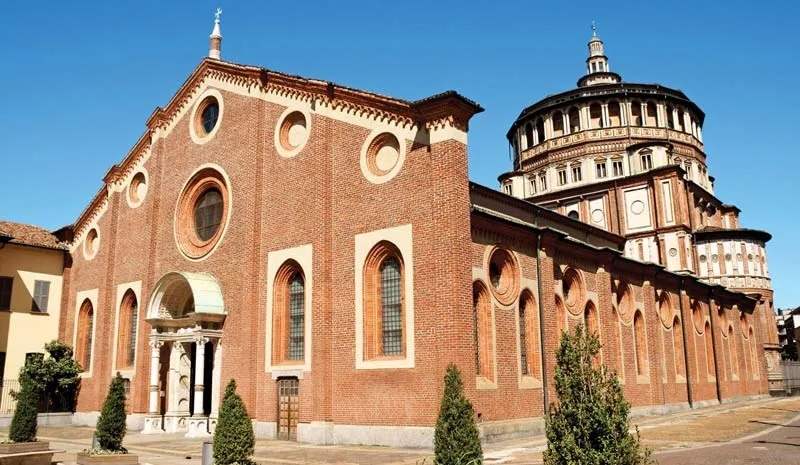
\includegraphics[scale=0.33]{img/churchmilan}
  \caption{米兰圣母玛丽亚感恩大教堂}
 \label{fig:church-Milan}
\end{figure}

塔尔塔利亚失去了布雷西亚的教授工作,他在贫穷和愤恨中走完了自己的一生。卡尔达诺的誓言似乎冥冥中笼罩着他。1560年他的长子被控毒杀不忠的妻子被判处死刑。卡尔达诺彻底被丧子之痛击倒了,他从米兰搬到布雷西亚住。1565年,卡尔达诺再次遭受打击,得意门生费拉里被他姐姐毒杀。卡尔丹诺沉迷赌博和占星术,他因推算出了耶稣的星象,被教会判处大逆不道,于1570年锒铛入狱。出狱后他移居罗马,在生命的最后一年出版了一本自传。在自传中,他不断重复丧子之痛,吹嘘自己的成就,但只用一句话轻描淡写地谈到了塔尔塔利亚。我们今天对这段历史的还原主要来自塔尔塔利亚的《新问题新发明》,以及他和中间人书商、卡尔达诺、费拉里往来的信件。

\begin{figure}[htbp]
 \centering
 \subcaptionbox{塔尔塔利亚\label{fig:tartaglia}}{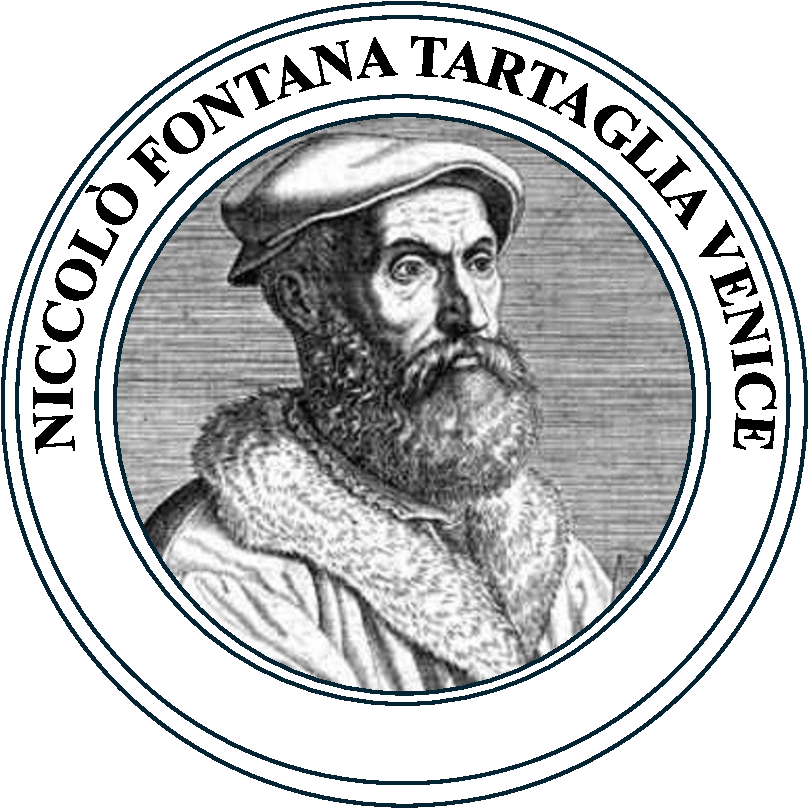
\includegraphics[scale=0.35]{img/tartaglia-coin}}
 \subcaptionbox{卡尔达诺\label{fig:cardano}}{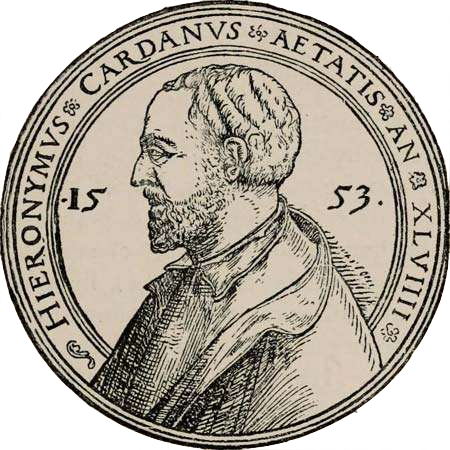
\includegraphics[scale=0.3]{img/Cardano}}
 \caption{塔尔塔利亚与卡尔达诺}
\end{figure}

今天,人们把三次方程的求根公式叫做卡尔达诺——塔尔塔利亚公式,简称卡尔达诺公式。此外塔尔塔利亚还在1546年发表过弹道学著作,第一个给出了弹道表格。1543年他第一个把欧几里得《原本》翻译成意大利语出版,此外他把阿基米德的一些著作翻译成意大利语。除了明显的缺陷外,卡尔达诺是一名百科全书式的学者。他是第一个对斑疹伤寒做出临床描述的人,数学上的贡献涵盖代数、概率论。他还发明了万向轴,被称作卡尔达诺轴。莱布尼茨评价到:“尽管有缺点,他是个伟人;但如果没有这些缺点,他将是无与伦比的。”

\section{三次方程}

与通常的观点不同,复数\underdot{不是}在解二次方程的过程中,而是在解三次方程的过程中被意外发现的。高中数学课上会给出卡尔达诺公式。本节将利用代数与几何两种方法推导这个公式。

\begin{figure}[htbp]
  \centering
  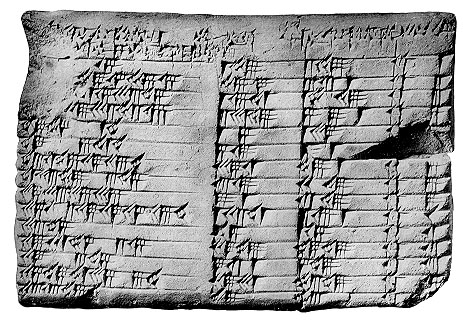
\includegraphics[scale=0.33]{img/plimpton322}
  \caption{编号普林普顿322的古巴比伦泥板,内容为勾股数表,约公元前2020年。藏于哥伦比亚大学。二十世纪二十年代由乔治·亚瑟、普林普顿捐赠给哥伦比亚大学。}
 \label{fig:plimpton322}
\end{figure}

%% https://personal.math.ubc.ca/~cass/courses/m446-03/pl322/pl322.html
我们是从古巴比伦泥板上了解到二次方程的早期历史的。如\cref{fig:plimpton322}所示,这是藏于哥伦比亚大学的一块泥板,编号为普林普顿322。这块泥板上的楔形文字内容很有特点,德国科学史家诺伊格鲍尔和萨克斯将发现它竟然是一张勾股数表。根据第1章给出的古巴比伦计数系统,我们很容易看出最后一列是编号$1, 2, 3, \dotsc, 15$,其中5,6,15三个数字损毁了。同样右边第二列也是编号。左边第二列的表头注明是直角三角形的底,从上到下转换为十进制依次是:$119, 3367, 4601, \dotsc, 1771, 56$,其中最后的56损毁了,并且有两处错误。左边第三列的表头注明是直角三角形的斜边,从上到下转换成十进制依次为:$169, 4825, 6649, \dotsc, 3229, 106$,同样最后的数字有错并且损毁了。左边第一列的数字最难破译,古巴比伦此时还没有使用零,也没有小数点。科学家们将其破译并转换为十进制数字,依次为:$1.9834\dotso, 1.94916\dotso, 1.9188\dotso$直到$1.43024\dotso, 1.38716\dotso$。60进制小数转换为10进制通常会除不尽(见\cref{thm:finite-decimal}),因此我们增加了省略号。如果我们记直角三角形的底为$w$,斜边为$d$,高为$h$,科学家们发现第一列的数字是$\dfrac{d^2}{h^2}$,根据勾股定理它等于$\dfrac{d^2}{d^2 - w^2}$。例如第一行:$d = 169, w = 119$,计算可得:

\[
\frac{d^2}{d^2 - w^2} = \frac{169^2}{169^2 - 119^2} = 1.9843\dotso
\]

%% https://engelsbergideas.com/notebook/the-brilliance-of-babylonian-mathematics/
正好是第一行中的第一个数字。这个勾股数表证实古巴比伦人知晓勾股定理(尽管没有定理的证明),并将其应用于计算。随着更多楔形文字泥板的出土,科学家们还发现了勾股定理的“配套练习题”。其中一道题目说:“已知长方形的面积和对角线,求长方形的两个边长。”这道典型的土地丈量问题相当于解方程:

\[
\begin{cases}
  ab = s \\
  a^2 + b^2 = d^2
\end{cases}
\]

其中$s$是面积,$d$是对角线。将$b = \dfrac{s}{a}$代入第二式,就得到关于$a^2$二次方程$(a^2)^2 - d^2 a^2 + s^2 = 0$。当时还没有代数符号系统,古巴比伦人解二次方程的过程是通过文字描述的。初中课堂上通常会在介绍求根公式前,学习用“配方法”(complete square)解二次方程。这本质上也是一种代数解法。阿拉伯数学家花拉子密在他的《代数学》中还遵循古希腊传统给出了二次方程的几何解释\footnote{即Hisab al-jabr w'al-muqabala,见第\ref{sec:Khwarizmi}节}。如果$a \ne 0$,我们可以把一般二次方程$ax^2 + bx + c = 0$的二次项系数化成1,然后把常数项移到右侧,得到$x^2 + \dfrac{b}{a}x = -\dfrac{c}{a}$。令$p = \dfrac{b}{a}, q= -\dfrac{c}{a}$,我们要通过几何方法解方程$x^2 + px = q$。如果$p > 0$,\cref{fig:quadratic1}给出了方程左侧的几何意义。$q$相当于一个正方形的面积$x^2$加上一个长$p$宽$x$的矩形面积。

\begin{figure}[htbp]
  \centering
  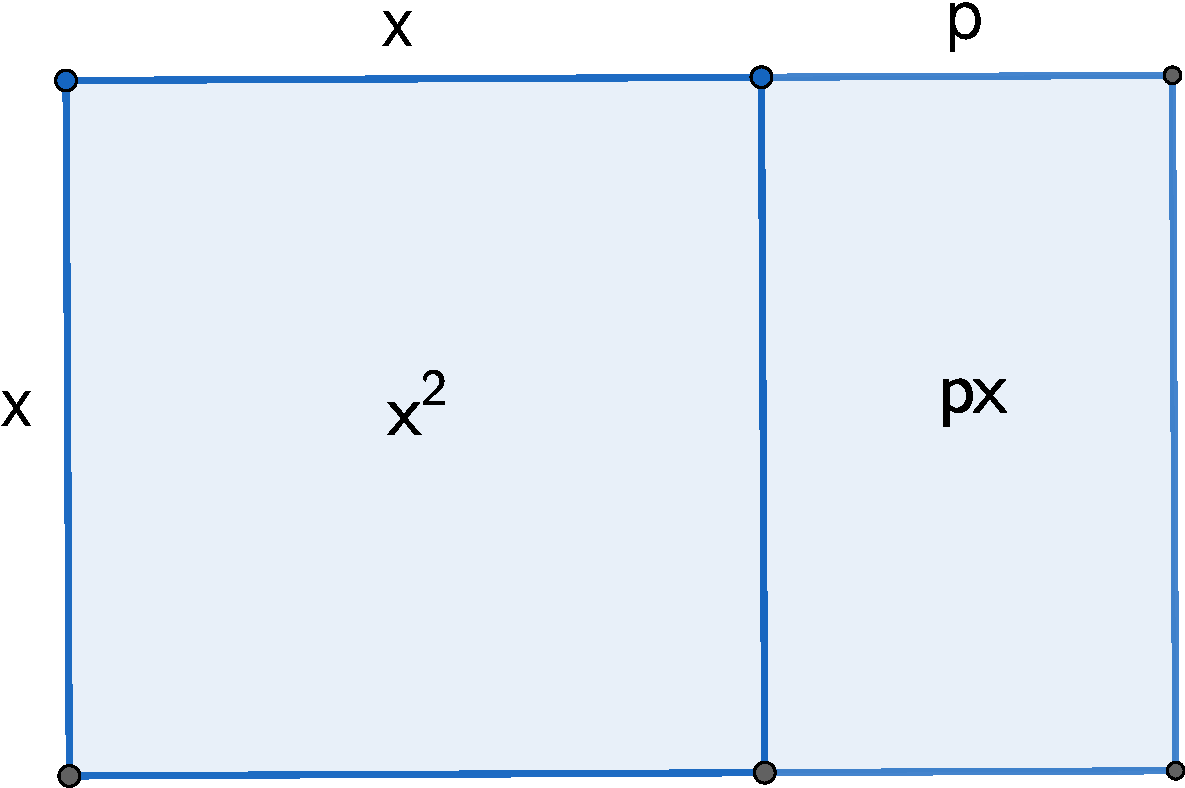
\includegraphics[scale=0.5]{img/quadratic1}
  \caption{$x^2 + px$的几何意义:正方形与长方形的面积和}
 \label{fig:quadratic1}
\end{figure}

配方法的几何意义是把矩形切分成两个同样的长$\dfrac{p}{2}$宽$x$的小矩形(见\cref{fig:quadratic2}左侧),然后把其中一个移动到正方形的下方,再补上一个边长为$\dfrac{p}{2}$的小正方形(见\cref{fig:quadratic2}右侧的黑色正方形)拼成一个边长为$x + \dfrac{p}{2}$的大正方形。左右两边图形中的白色面积相等,即:

\begin{align*}
 (x + \frac{p}{2})^2 &= q + (\frac{p}{2})^2 &&\text{大正方形面积等于白色部分加黑色部分} \\
 x + \frac{p}{2} &= \pm \sqrt{q + (\frac{p}{2})^2} &&\text{两边开方} \\
 x &= -\frac{p}{2} \pm \sqrt{q + \frac{p^2}{4}} \\
 x &= -\frac{b}{2a} \pm \sqrt{-\frac{c}{a} + \frac{b^2}{4a^2}} &&\text{代入}p = \frac{b}{a}, q= -\frac{c}{a} \\
 x &= \frac{-b \pm \sqrt{b^2 - 4ac}}{2a}
\end{align*}

\begin{figure}[htbp]
  \centering
  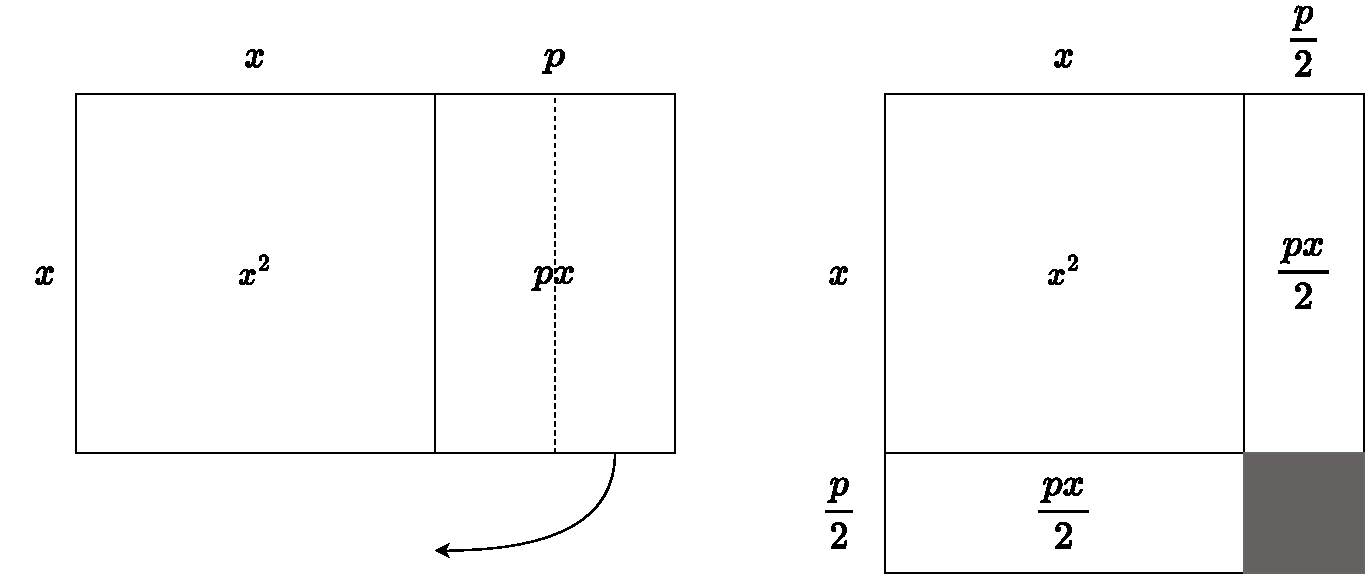
\includegraphics[scale=0.5]{img/quadratic2}
  \caption{$x^2 + px$的几何意义:正方形与长方形的面积和}
 \label{fig:quadratic2}
\end{figure}

这就是常见的一元二次方程求根公式。但在花拉子密时代负数还没有被接受,因此当一次项为负时就需要给出$x^2 - px = q$的几何解释;当常数项为负时需要给出$x^2 - q = px$的几何解释(见\cref{qn:geometric-quadratic})。卡尔达诺在《大术》中遵循了这样的传统,同时给出了三次方程的代数解法和几何解释。我们先介绍代数解法。对于一般三次方程$a_3x^3 + a_2x^2 + a_1x + a_0 = 0, a_3 \ne 0$,首先两边同时除以$a_3$把三次项系数化为1,即$x^3 + \dfrac{a_2}{a_3} x^2 + \dfrac{a_1}{a_3} x + \dfrac{a_0}{a_3}$。重新命名系数为$x^3 + ax^2 + bx + c = 0$。大约在十四世纪末,意大利佛罗伦萨的数学家就发现可以通过变量替换$x = y - \dfrac{a}{3}$把二次项消去:

\begin{align*}
(y - \frac{a}{3})^3 + a(y - \frac{a}{3})^2 + b(y - \frac{a}{3}) + c &= 0  \\
y^3 -\cancel{ay^2} + \frac{a^2}{3}y - \frac{a^3}{27} + \cancel{ay^2} - \frac{2a^2}{3}y + \frac{a^3}{9} + by - \frac{ab}{3} + c &= 0 && \text{二项式展开} \\
y^3 + (b - \frac{a^2}{3})y + \frac{2a^3}{27} - \frac{ab}{3} + c &= 0 \\
y^3 + py + q = 0
\end{align*}

其中$p = b - \dfrac{a^2}{3}, q = c + \dfrac{2a^2}{27} - \dfrac{ab}{3}$。由于当时人们不接受负数,根据$p, q$的正负,这种“缺二次项”的三次方程共有三种形式:

\begin{align}
y^3 + py &= q \label{eq:cubic-linear} \\
     y^3 &= py + q \label{eq:cubic-complex} \\
y^3 + q &= py
\end{align}

其中费罗独立发现的是\cref{eq:cubic-linear}形式的解,而\cref{eq:cubic-complex}形式的解直接导致了复数的发现。我们不妨以$y^3 = py + q$为例继续推导求根公式。令$y = u + v$,则方程左侧化为:

\begin{align*}
y^3 = (u + v)^3 &= u^3 + 3u^2v + 3uv^2 + v^3 && \text{二项式展开} \\
  &= u^3 + v^3 + 3uv(u + v) \\
  &= u^3 + v^3 + 3uvy && \text{代入} y = u + v \\
  &= (3uv)y + (u^3 + v^3) = py + q && \text{左边等于右边}
\end{align*}

由待定系数法知:

\[
\begin{cases}
  3uv = p \\
  u^3 + v^3 = q
\end{cases}
\]

这相当于关于$u, v$的二元方程组。从第一个方程中得到:$v = \dfrac{p}{3u}$,代入第二个方程得:

\[
u^3 + (\frac{p}{3u})^3 = q
\]

这实际上是一个关于$u^3$的二次方程:$(u^3)^2 - qu^3 + (\dfrac{p}{3})^3 = 0$,利用二次方程求根公式得到:

\[
u^3 = \frac{q}{2} \pm \sqrt{(\frac{q}{2})^2 - (\frac{p}{3})^3}
\]

注意到$u, v$在上面的二元方程组中是完全对称的,$v^3$必然具有同样的形式。我们不妨让它们分别取这两个根:

\[
\begin{cases}
u^3 = \dfrac{q}{2} + \sqrt{(\dfrac{q}{2})^2 - (\dfrac{p}{3})^3} \\
v^3 = \dfrac{q}{2} - \sqrt{(\dfrac{q}{2})^2 - (\dfrac{p}{3})^3}
\end{cases}
\]

这样它们满足$u^3 + v^3 = q$。最后由$y = u + v$,我们得到方程的根:

\be \label{eq:cardano}
y = u + v = \sqrt[3]{\frac{q}{2} + \sqrt{(\frac{q}{2})^2 - (\frac{p}{3})^3}} + \sqrt[3]{\frac{q}{2} - \sqrt{(\frac{q}{2})^2 - (\frac{p}{3})^3}}
\ee

这就是高中数学课上介绍的卡尔达诺公式。我们进一步可以用$x = y - \dfrac{a}{3}$求出未知数$x$。与此对照,我们接下来用几何法解三次方程$y^3 + py = q$。如\cref{fig:cube-decompose}所示,把一个边长为$r$的大正方体切分为5部分:左前下角的边长为$r-s$的小正方体;右后上角的边长为$s$的小正方体;三个长$r$宽$r-s$高$s$的长方体,分别位于左上、右前、后下。大正方体的体积等于这5部分的体积之和,即:

\begin{figure}[htbp]
  \centering
  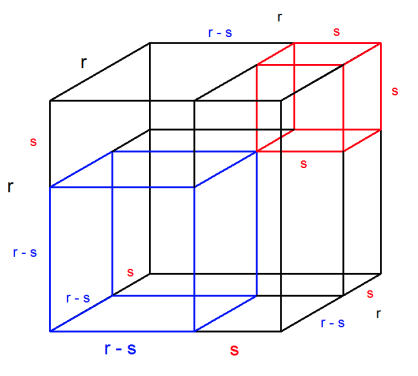
\includegraphics[scale=0.4]{img/cube-decompose}
  \caption{把边长为$r$的正方体切分成5部分}
 \label{fig:cube-decompose}
\end{figure}

\begin{align*}
r^3 = (r-s)^3 + s^3 + 3rs(r-s)  &&\text{两个正方体加三个长方体} \\
(r-s)^3 + 3rs(r-s) = r^3 - s^3
\end{align*}

令$p = 3rs, q = r^3 - s^3$,则上述等式就是$(r-s)^3 + p(r-s) = q$。显然$y = r - s$就是方程$y^3 + py = q$的一个解。所以只要根据$p, q$找到合适$r, s$就能解出三次方程了。由$p = 3rs$得$s = \dfrac{p}{3r}$,代入$q = r^3 - s^3$得到方程:

\[
r^3 - (\frac{p}{3r})^3 = q
\]

这本质上是一个关于$r^3$的二次方程$(r^3)^2 - qr^3 - (\dfrac{p}{3})^3 = 0$,利用二次方程求根公式得到:

\[
r^3 = \frac{q}{2} + \sqrt{(\frac{q}{2})^2 + (\frac{p}{3})^3}
\]

对称地可以求出$s^3$:

\[
s = -\frac{q}{2} + \sqrt{(\dfrac{q}{2})^2 + (\dfrac{p}{3})^3}
\]

最终求得未知数$y = r - s$:

\[
y = r - s = \sqrt[3]{\frac{q}{2} + \sqrt{(\frac{q}{2})^2 + (\frac{p}{3})^3}} - \sqrt[3]{\frac{q}{2} + \sqrt{(\frac{q}{2})^2 + (\frac{p}{3})^3}}
\]

和代数法推出的卡尔达诺公\cref{eq:cardano}对比,只有$p$的正负号不同,这是由于方程$y^3 + py = q$和$y^3 = py + q$中$p$的符号相反。我们可以尝试用卡尔达诺公式解方程$x^3 = 6x + 9$。

\begin{align*}
x &= \sqrt[3]{\frac{9}{2} + \sqrt{(\frac{9}{2})^2 - (\frac{6}{3})^3}} + \sqrt[3]{\frac{9}{2} - \sqrt{(\frac{9}{2})^2 - (\frac{6}{3})^3}} \\
  &= \sqrt[3]{\frac{9}{2} + \sqrt{\frac{81 - 32}{4}}} + \sqrt[3]{\frac{9}{2} - \sqrt{\frac{81 - 32}{4}}} \\
  &= \sqrt[3]{\frac{9}{2} + \frac{7}{2}} + \sqrt[3]{\frac{9}{2} - \frac{7}{2}} \\
  &= \sqrt[3]{8} + \sqrt[3]{1} = 2 + 1 = 3
\end{align*}

验证的确有$3^3 = 27 = 6 \times 3 + 9$。三次方程的公式解是数学上的重大突破,人们迫不及待地用它来解决各种个样的问题。可是有些方程的结果却令人大惑不解,其中最著名的例子是方程$x^3 = 15x + 4$。通过观察$x = 4$是方程的一个解:$4^3= 64 = 60 + 4 = 15 \times 4 + 4$。但卡尔达诺公式给出的结果是:

\begin{align*}
x &= \sqrt[3]{2 + \sqrt{2^2 - 5^3}} + \sqrt[3]{2 - \sqrt{2^2 - 5^3}}  \\
  &= \sqrt[3]{2 + \sqrt{-121}} + \sqrt[3]{2 - \sqrt{-121}}
\end{align*}

\index{数学家!邦贝利}
竟然在二次根号下出现了负数。以前在解二次方程时,如果判别式的值为负,人们可以说“无解”。但这个方程明明有一个解$x = 4$,并非“无解”。人们必须正视这个问题。卡尔达诺不知道如何解答,他在《大术》中评论道:“这些数即微妙又无用。”在这个问题上取得突破的是意大利数学家邦贝利(Rafael Bombelli, 1526~1572)。邦贝利设想把$\sqrt[3]{2 \pm \sqrt{-121}}$化简成$a \pm b\sqrt{-1}$的形式。这样卡尔达诺公式的两项加起来就是:

\[
\sqrt[3]{2 + \sqrt{-121}} + \sqrt[3]{2 - \sqrt{-121}} = a + b\sqrt{-1} + a - b\sqrt{-1} = 2a = 4
\]

这样就确定出$a = 2$。接下来通过待定系数法确定$b$的值。邦贝利假设$(\sqrt{-1})^2 = -1$,把两边乘3次方:

\begin{align*}
2 + \sqrt{-121} &= (2 + b\sqrt{-1})^3 \\
  &= 8 + 12b\sqrt{-1} - 6b^2 - b^3\sqrt{-1} && \text{二项式展开} \\
  &= (8 - 6b^2) + (12b - b^3)\sqrt{-1}
\end{align*}

由$2 = 8 - 6b^2$得出$b = \pm 1$;把1代入$(12b - b^3)\sqrt{-1}$得$11\sqrt{-1}$。平方后可验证:$(11\sqrt{-1})^2 = -121$。于是有$\sqrt[3]{2 + \sqrt{-121}} = 2 + \sqrt{-1}$。对于$b = -1$,邦贝利接着通过两边乘3次方验证了$\sqrt[3]{2 - \sqrt{-121}} = 2 - \sqrt{-1}$也成立。他对这个结果非常满意,在1572年出版的《代数》一书中写道:“起初,我感到这样处理更像是诡辩而非真理,但我不断探寻,直至找到证明。”\cite{OMerino-2006}邦贝利的数学观点远远超越了他的时代。当时负数尚未被欧洲接受,邦贝利在《代数》中不仅正确地定义了正负数之间的运算规则,还给出了复数的计算规则。他称$\sqrt{-n}$为“负的正”(plus of minus)称$-\sqrt{-n}$为“负的负”(minus of minus),然后写道\cite{MacTour-Bombelli}:

\begin{quotation}
负的正乘以负的正为负,即:$\sqrt{-n} \times \sqrt{-n} = -n$;

负的正乘以负的负为正,即:$\sqrt{-n} \times -\sqrt{-n} = n$;

负的负乘以负的正为正,即:$-\sqrt{-n} \times \sqrt{-n} = n$;

负的负乘以负的正为负,即:$-\sqrt{-n} \times -\sqrt{-n} = -n$;
\end{quotation}

非常遗憾的是,邦贝利原来准备出版五卷本《代数》,但1572年出版了前三卷后他就去世了。剩余的两卷本草稿直到1923年才被发现于意大利博洛尼亚的图书馆。当时的人们并没有相信并接受邦贝利的观点,数学界基本排斥$\sqrt{-1}$。在接下来的200年间,即使有少数学者如沃利斯尝试赋予复数涵义,但大多数人要么怀疑,要么忽视了邦贝利的计算规则。直到1770年,大数学家欧拉仍然在他的著作中“证明”$\sqrt{-2} \times \sqrt{-3} = \sqrt{6}$,我们今天看到这个结论会感到很意外\footnote{欧拉实际上用符号$\sqrt{6}$表示6的一对平方根$\pm\sqrt{6}$,类似地$\sqrt{-2}$表示-2的一对平方根$\pm\sqrt{-2}$,$\sqrt{-3}$表示-3的一对平方根$\pm\sqrt{-3}$,这样欧拉的本意是想表示$\pm \sqrt{-2} \times \pm \sqrt{-3} = \pm \sqrt{6}$的所有组合}。也有人高度评价邦贝利的工作,莱布尼茨说他是“杰出的分析艺术大师。”今天人们称邦贝利为“虚数之父”。

\begin{figure}[htbp]
  \centering
  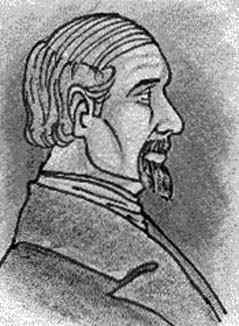
\includegraphics[scale=0.4]{img/Bombelli}
  \caption{拉斐尔·邦贝利,1526~1572}
 \label{fig:Bombelli}
\end{figure}

邦贝利的方法中使用了$a + b\sqrt{-1}$的形式。第一个使用$a + \sqrt{-b}$的是卡尔达诺,但是他否定了自己的结论。在《大术》第37章,卡尔达诺给出了这样的一个问题:把10分成两部分,使得它们的乘积是40。列方程就是:

\[
\begin{cases}
x + y = 10 \\
xy = 40
\end{cases}
\]

消元可得一元二次方程$x(x-10) = 40$。我们知道,把10分成两部分最大的乘积是$5 \times 5 = 25$,所以乘积40是不可能的(也可以这样思考:把一根长20厘米的绳子围成矩形,面积最大时是边长为5的正方形,此时面积是25平方厘米)。卡尔达诺写道:

\begin{quotation}
显然这是不可能的。尽管如此,我们可以这样做:我们把10均分成两个5,平方是25。减去40,如果你希望的话,得-15。把-15的平方根加上、减去5得到的两个数的乘积就是40。因此这两个数是$5 + \sqrt{-15}$和$5 - \sqrt{-15}$。

尽管匪夷所思,把两个数$5 + \sqrt{-15}$和$5 - \sqrt{-15}$相乘得$25-(-15)$,因此它们的积是40。
\end{quotation}

卡尔达诺的方法是把10分成$5 + x$和$5 - x$,让它们的积是40。利用平方差公式$(5 + x)(5 - x) = 25 - x^2 = 40$,因此$x^2 = -15$。这样推出解为$x_{1, 2} = 5 \pm \sqrt{-15}$。正是由于其在现实应用,特别是在一元二次方程应用中的不合理性,卡尔达诺以及同时代的大多数人舍弃了复数答案。但是邦贝利意识到在三次方程的\underdot{合理}应用中,作为中间结果的复数有其存在价值。那么“虚数”这个名字是怎么来的呢?这要“归功”于笛卡尔。笛卡尔在1637年发表的《谈谈方法》的附录《几何学》中创建了解析几何。方程的根对应曲线间的交点或曲线与坐标轴的零点。尽管当时人们没有认识到代数基本定理,笛卡尔还是敏锐地洞见到方程根的个数等于方程的次数。但是从几何上的观点上看,某些曲线不和$x$轴相交,或者曲线间不相交。面对这些几何上不可能的构造,笛卡尔认为它们的交点或零点是虚构的。“虚数”一词就来自笛卡尔文中的imaginary,在英文中它同时还有想象的涵义。笛卡尔写道:“对于任何方程,人们可以想象(imagine)有着和次数同样多的根,但在很多情况下,这些根对应的值并不存在。”

我们今天广泛使用符号$i$作为虚数单位。这个符号是欧拉选定的。它是imaginary的首字母。笛卡尔的态度反映了当时大多数人的观点。数学家们并不喜欢虚构、想象这些涵义。其中一个原因是$\sqrt{-n}$带来了混乱和歧义。例如常见的运算规则$\sqrt{ab} = \sqrt{a}\sqrt{b}$还成立么?有人指出这样的问题:

\begin{align*}
70 &= \sqrt{4900} = \sqrt{(-100)\times(-49)} = \sqrt{-100}\sqrt{-49} \\
   &= (10i)(7i) = 70 \times (-1) = -70
\end{align*}

这样就出现了$70 = -70$的矛盾结论(见\cref{qn:sqrt-of-product})。复变函数之父柯西建议拒绝符号$\sqrt{-1}$,高斯对$i$也不满意,建议取个新名字。但他的建议太晚了,$i$已经被广泛使用,直到今天。

\section{佚名数学家}

为了让复数真正进入数的大家族得到承认,必须解决它的意义问题。并且这种意义不能是牵强附会的空中楼阁,它必须是自然的、让人信服的并且能解决真正的问题。1673年,微积分的先驱者英国数学家沃利斯试图给出复数的几何解释,但是他和成功失之交臂。沃利斯是数轴的发明者,他正是利用数轴作为武器,尝试解方程$x^2 + 2bx + c^2 = 0$。根据二次方程求根公式,方程的两个根是:$x_{1,2} = -b \pm \sqrt{b^2 - c^2}$。如\cref{fig:wallis1}所示,沃利斯在数轴上找到$-b$,然后以这点为垂足构造一左一右两个直角三角形,其高为$c$、斜边为长$b$。根据勾股定理,另一直角边长为$a = \sqrt{b^2 - c^2}$。所以点$-b$左右两侧距离$a$的两个点就是$x_{1,2}$。

\begin{figure}[htbp]
  \centering
  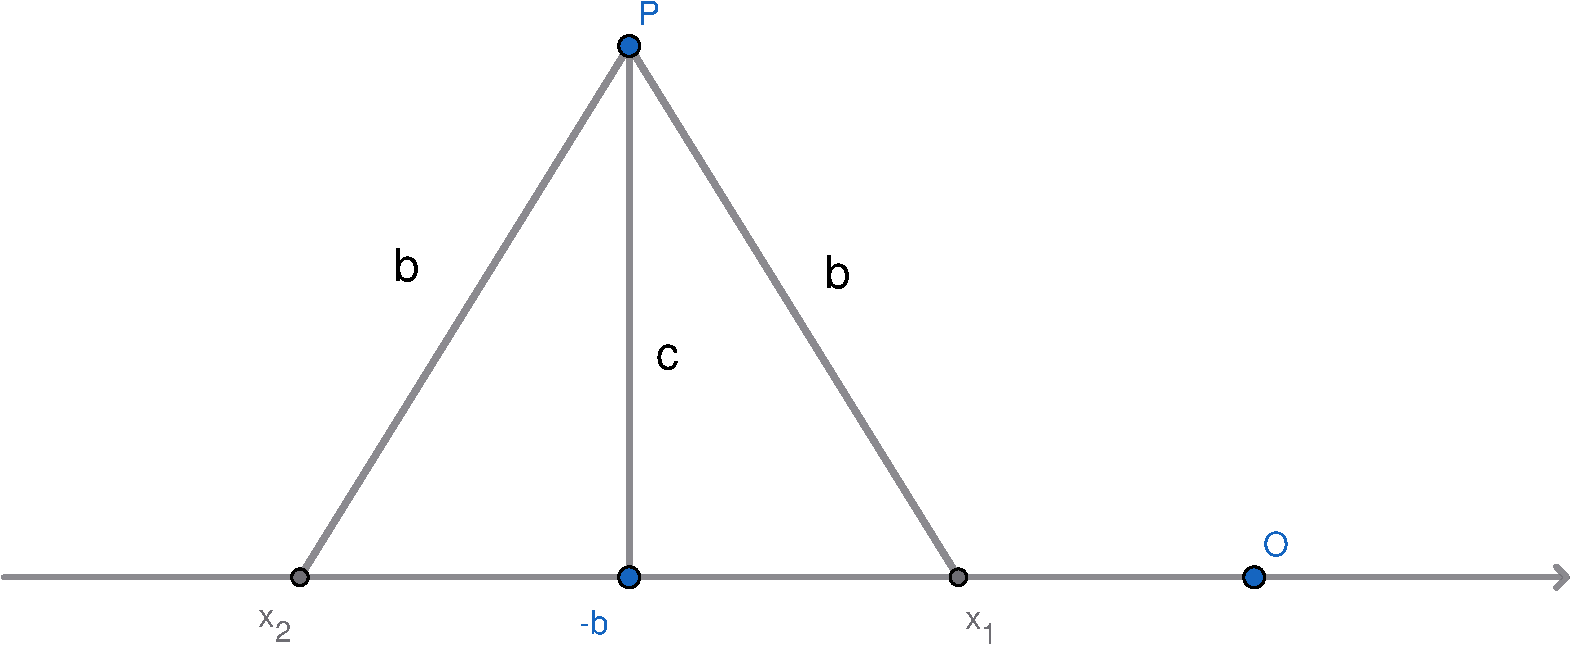
\includegraphics[scale=0.33]{img/wallis1}
  \caption{根$x_{1,2} = -b \pm \sqrt{b^2 - c^2}$在数轴上的位置}
 \label{fig:wallis1}
\end{figure}

到此为止一切正常。接着沃利斯不断增大$c$的值,两个根$x_{1,2}$越来越靠近$-b$点。当$c = b$时两个根重合了。如果继续增大$c$会怎样呢?沃利斯绘制出了这样一幅图,如\cref{fig:wallis2}所示。

\begin{figure}[htbp]
  \centering
  \subcaptionbox{沃利斯认为$-b \pm i\sqrt{c^2-b^2}$所在的位置\label{fig:wallis2}}{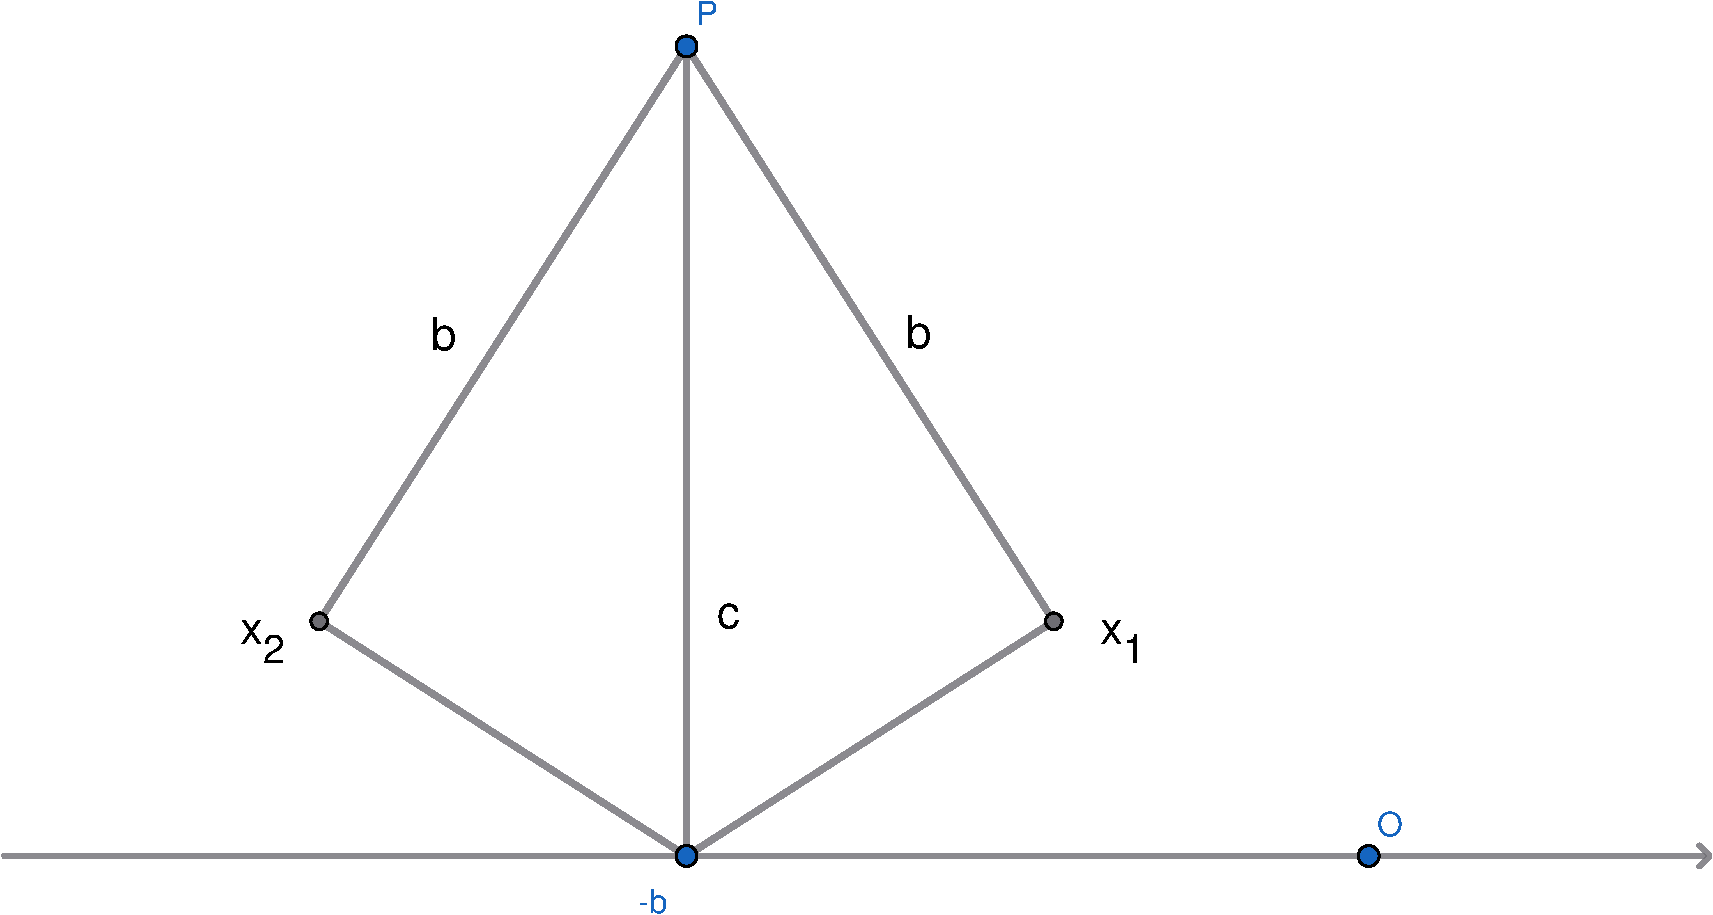
\includegraphics[scale=0.33]{img/wallis2}}
  \subcaptionbox{实际上$-b \pm i\sqrt{c^2-b^2}$在复平面上的位置\label{fig:wallis3}}{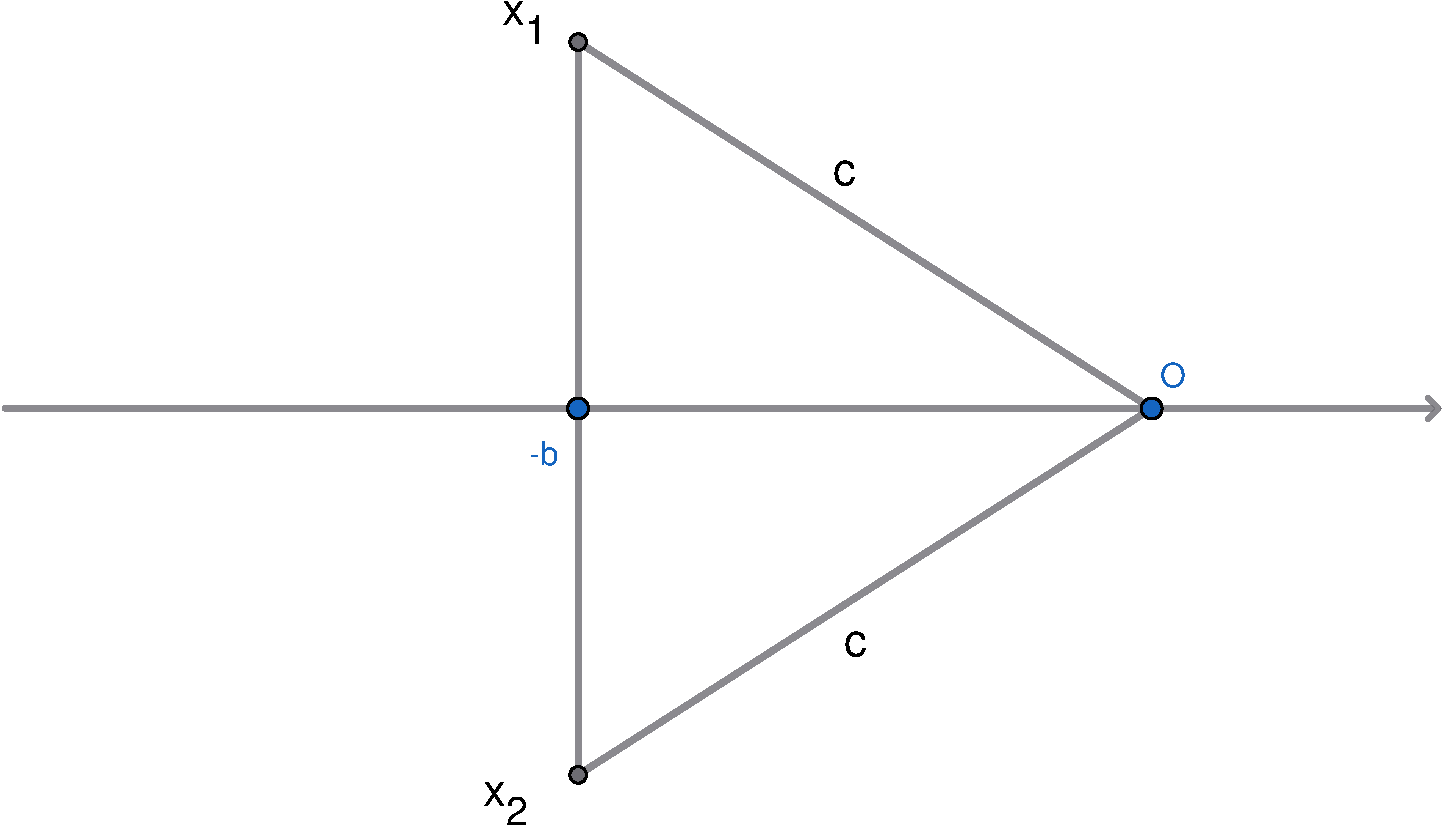
\includegraphics[scale=0.33]{img/wallis3}}
  \caption{方程$x^2 + 2bx + c^2 = 0$的两个根}
\end{figure}

\index{数学家!韦塞尔}
这已经非常接近真相了。沃利斯认为此时$c$成为斜边,一条直角边是$b$,另一直角边是$\sqrt{c^2 - b^2}$,但它们仍然在点$-b$的左右两侧。实际上沃利斯只要把左右两侧换成上下就能触摸到复平面了。这真令人惋惜。在历史上第一成功解决了复数几何意义的人是丹麦-挪威数学家卡斯帕尔·韦塞尔(Caspar Wessel,1745~1818)。1797年3月10日,韦塞尔向丹麦皇家科学提交了他的著作,题为《论方向的解析表示——主要应用于平面和球面多边形求解的尝试》。他成功地把复数$a + bi$表示为平面直角坐标系中从原点指向坐标$(a, b)$的线段(即向量),并且定义了向量间的代数计算规则,包括加法和乘法。从几何的角度,加法规则相当于“平行四边形”原理;乘法相当于把线段的长度相乘,然后把各自相对于横轴的角度相加。韦塞尔的论文于两年后发表。非常遗憾的是,韦塞尔的职业是一名测量员而非知名数学家,并且论文的语言是丹麦语,当时并未引起广泛的关注。韦塞尔的名字被大多数人忽略了,直到约100年后的1895年,他的工作才重新引起人们重视。挪威数学家索菲斯·李重新发表了韦塞尔的论文。更加匪夷所思的是,1806年,一个年轻人重新独立发现了复平面和复数的几何意义,但没有人知道他的名字。

\subsection{佚名作者阿尔冈}
\index{数学家!阿尔冈}
1806年金秋,一位年轻人敲开了法国科学院院士数学家勒让德家的大门。他十分紧张,勒让德被认为是欧拉最好的弟子,拉格朗日的接班人。拿破仑重建科学院后,任命勒让德为数学部的负责人,法国最高学府巴黎综合工科学校的主考官。这位年轻人做了简单的自我介绍,由于紧张,他甚至忘记了介绍自己的名字。他恭敬地把自己的一篇研究手稿交给了勒让德,恳请他指正。年轻人没有仔细向勒让德解释他的目的,但是当被问起论文的内容时,他立刻兴奋起来了。“哦,尊敬的院士先生”,年轻人说:“这是一篇关于虚数的研究工作,我发现虚数其实是有意义的,它就像其它的数那样真实!只要我们把它们看成是线段,就会发现……”面对滔滔不绝的年轻人,勒让德一脸狐疑。他只好打断了这个年轻人。“我现在很忙,不过我答应有时间读一读你的文章,我们今天先到这里吧。”在大门关闭前年轻人再次恳请勒让德:“院士先生,我非常期待您的批评指正。”

送走了这位年轻人,勒让德很快就忙于其它研究和科学院的事务了。直到几周后,勒让德偶然看到了放在案头的几张纸,题目是《关于在几何构造中表示虚数的一种方法的论述》。这是谁送来的?哦,想起来了,那个年轻人叫什么来着?好像记不清了,不管怎样,勒让德读了下去。出乎意料的是,勒让德一旦开始读就立刻被这篇文章吸引住了。绝对出人意料的创新想法,行云流水般的论述,扎实的计算,精确的结论,把数、几何、三角函数完美地结合在一起。勒让德决定马上联系一下这位小伙子,和他深入讨论。可他翻遍了论文的前前后后,也没有找到任何姓名、地址。怎么会这样呢?也许这位年轻人过两天会再次登门拜访吧?勒让德决定等一等。一天、两天……从深秋等到初冬,转眼巴黎已经飘下了第一场雪。可年轻人再也没有出现。这位年轻人会不会直接在期刊上发表他的论文?这样我就能找到他讨论了。勒让德跑到图书馆检查了过去几个月的各种数学期刊,但再次让他失望。也许当天勒让德的态度让这位年轻人心灰意冷,放弃了这个研究。11月2日,勒让德把这篇论文寄给了他的朋友与合作者数学家弗朗索瓦·弗朗塞,并附上了一小段评论,他称赞了那位不慕虚荣热爱学术的年轻人,并认为尽管是草稿,但是具有足够的创新性。

弗朗索瓦·弗朗塞主要研究偏微分方程,尽管他的工作经常得到法国科学院的赞誉,但很少在生前发表。1810年弗朗塞死后,他的兄弟雅克·弗朗塞在整理遗稿时发现了这篇关于复数的论文,并于1813年9月以题目《新的位置几何学原理及虚数符号的解释》发表。雅克·弗朗塞展示了一个真正学者的风范,他没有把这个成果据为己有。在论文的结尾他指出这些想法来自一位不知名的数学家,并恳请这位数学家站出来以得到应有的荣誉。雅克·弗朗塞的这篇论文发表在热尔岗的著名期刊《数学年鉴》上不久,一位名叫阿尔冈的人来信声称他就是那位不知名的作者,并寄来了一份稍加修改的原稿,题目正是《关于在几何构造中表示虚数的一种方法的论述》。阿尔冈在其中加入了新的应用。这件本来就充满戏剧性的事件接下来引起了众多数学家的关注:雅克·弗朗塞、阿尔冈和数学家塞尔瓦在《数学年鉴》上展开了激烈的讨论。塞尔瓦认为必须用纯代数来处理复数,而雅克·弗朗塞和阿尔冈则主张几何表示法的有效性。阿尔冈接下来展示了复数几何表示法的威力——他一举证明了代数基本定理。以今天的眼光看,尽管有些瑕疵,但这是诸多证明中最清晰优美的一个。阿尔冈的工作是化时代的,但非常遗憾的是,我们不知道他究竟是谁!他在所有的论文中都仅仅署名“阿尔冈”。西方人的姓名是名字加姓氏,有的还有中间名。因此这相当于中国人仅仅署名“张”,究竟是张什么却一无所知。究竟是众多姓阿尔冈的人中的哪一位啊?我们只知道他1806年出现在巴黎,1813年发表的论文是从巴黎寄出的。有人猜测是他可能是让·罗伯特·阿尔冈,一位住在巴黎的会计员和业余数学家,但年龄对不上。1806年,勒让德描述的是一位年轻人,但彼时的让·罗伯特·阿尔冈已经38岁了\cite{MacTour-Argand}。

\index{阿尔冈图}
我们对这段历史的复原主要来自勒让德写给弗朗索瓦·佛朗塞的信,以及雅克·弗朗塞的论文。为了纪念阿尔冈的成就,今天我们把\cref{fig:Argand-diagram}叫做“阿尔冈图”(Argand diagram),它出现在全世界所有的中学课堂上。

\begin{figure}[htbp]
  \centering
  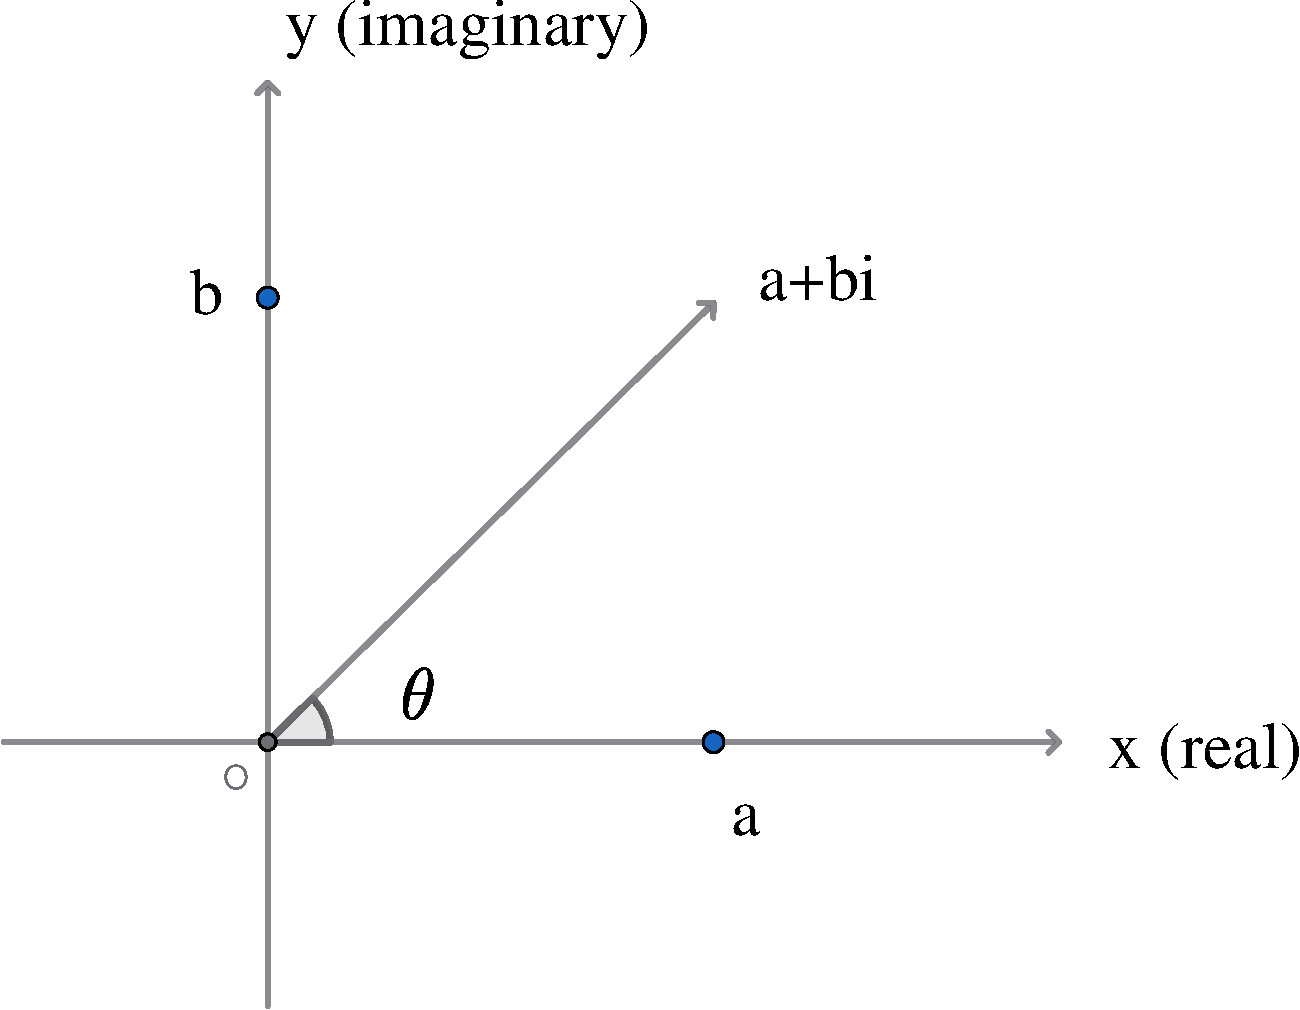
\includegraphics[scale=0.33]{img/argand-diagram}
  \caption{阿尔冈图}
 \label{fig:Argand-diagram}
\end{figure}

\subsection{复数的几何意义}

一图胜千言。我们可以立刻从阿尔冈图上看到复数$z$包含两个部分:实部$a$和虚部$bi$。虚轴创造性地垂直向上,实轴和虚轴彼此垂直,张成了复平面。复数被表示成了一个\underdot{向量},从原点指向复平面上坐标为$(a, b)$的点。画成一个带有箭头的线段,这个向量就是$a + bi$。虚数单位$i$不是任何实数,因为它根本不在实轴上。如果说实数轴上的任何数$a$乘以$-1$相当于“向后转”,变成指向另一侧的负数$-a$,那么$a$乘以$i$相当于“向左转$90\degree$”,变成虚轴上的$ai$;再次乘以$i$相当于再次“向左转$90\degree$”,变回实数轴上指向另一侧的$-a$。两次转$90\degree$相当于转$180\degree$,这就完美地解释了$i^2 = -1$。我们由勾股定理立刻看出向量$a + bi$所代表的线段的长度是$r = \sqrt{a^2 + b^2}$,它叫做复数$z$的模,记做$|z|$。向量与实轴张角为$\theta$,叫做复数的幅角,记做$arg(z)$。由三角函数的定义我们立刻知道复数的实部与虚部可以表示为:$a = r\cos\theta, b = r\sin\theta$,因此复数有两种等价的表示:

\[
a + bi = r\cos\theta + ir\sin\theta = r(\cos\theta + i\sin\theta)
\]

我们可以利用阿尔冈图进一步看出复数乘法的几何本质:

\begin{align*}
z_1z_2 &= r_1(\cos\theta_1 + i\sin\theta_1) \cdot r_2(\cos\theta_2 + i\sin\theta_2) \\
  &= r_1r_2(\cos\theta_1\cos\theta_2 - \sin\theta_1\sin\theta_2 + i(\sin\theta_1\cos\theta_2 + \cos\theta_1\sin\theta_2)) && \text{展开}, i^2 = -1 \\
  &= r_1r_2(\cos(\theta_1 + \theta_2) + i\sin(\theta_1 + \theta_2)) && \text{和角公式}
\end{align*}

\label{sec:proof-to-machin}
因此两个复数相乘,它们的模相乘,幅角相加。阿尔冈图可以说是数、几何、向量、三角函数完美融合的典范。为了展示复数具备的数形结合威力,我们给出麦钦公式的优美证明(见第\ref{sec:machin-formula}节)。用莱布尼茨公式计算圆周率的效率很低,为此人们提出了改进:

\[
\frac{\pi}{4} = \tan^{-1} \frac{1}{2} + \tan^{-1} \frac{1}{3}
\]

\begin{proof}
我们先证明这个改进的公式。复数$z = a + bi$的幅角$arg(z) = \tan^{-1}\dfrac{b}{a}$。上式右侧可以看作是两个幅角相加,它们分别对应复数:$z_1 = 2 + i, z_2 = 3 + i$。复数相乘时幅角相加,即:$arg(z_1 z_2) = arg(z_1) + arg(z_2)$。

\begin{align*}
z_1 z_2 &= (2+i)(3+i) = (6 - 1) + (2 + 3)i = 5 + 5i \\
arg(5 + 5i) &= arg(2+i) + arg(3+i) && \text{复数相乘幅角相加} \\
\frac{\pi}{4} &= \tan^{-1}\frac{5}{5} = \tan^{-1}\frac{1}{2} + \tan^{-1}\frac{1}{3} && \text{见\cref{fig:machin1}} \qedhere
\end{align*}
\end{proof}

\begin{figure}[htbp]
  \centering
  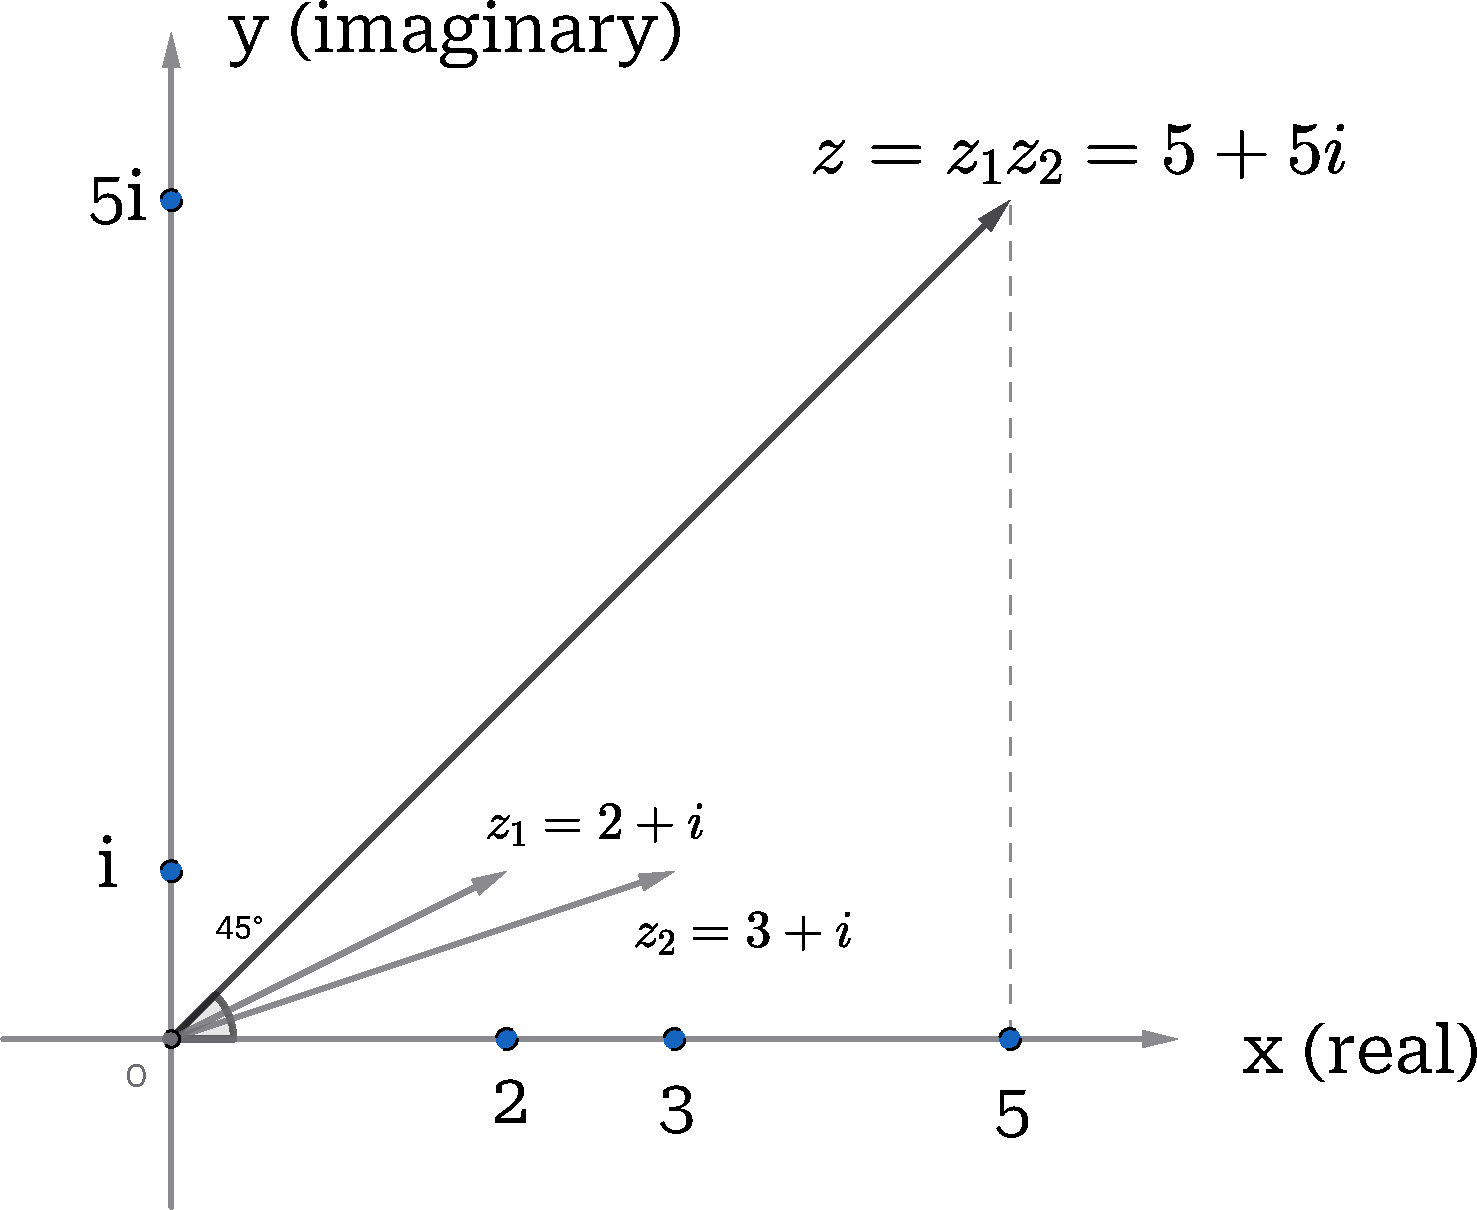
\includegraphics[scale=0.33]{img/machin1}
  \caption{$(2 + i)(3 + i) = 5 + 5i$}
 \label{fig:machin1}
\end{figure}

接下来证明麦钦公式:
\[
\frac{\pi}{4} = 4\tan^{-1} \frac{1}{5} - \tan^{-1} \frac{1}{239}
\]

\begin{proof}
令$z_1 = 5 + i, z_2 = 239 - i$。麦钦公式右侧幅角的4倍相当于$z_1^4$,我们构造复数乘积:

\begin{align*}
z &= z_1^4z_2 = (5+i)^4(239-i) \\
  &= (25 - 1 + 10i)^2(239 - i) && \text{完全平方公式} \\
  &= (24^2 - 100 + 480i)(239 - i) && \text{再次完全平方} \\
  &= 476 \times 239 + 480 + (480 \times 239 - 476)i && \text{展开} \\
  &= 114244 + 114244i
\end{align*}

$z$的幅角恰好是$\dfrac{\pi}{4}$
\end{proof}

这恐怕是麦钦公式最短最优美的证明。这个证明中还蕴含着一个复数的几何特性:如果复数$z = a + bi$的幅角是$\theta$,其中$b \ne 0$,则复数$a - bi$的幅角是$\tan^{-1}\dfrac{-b}{a} = -\theta$。记$\overline{z} = a - bi$为$z$的共轭复数。这样除以$a + bi$转动的角度相当于乘以$a - bi$所转动的角度。我们可以通过共轭复数方便地把除法转换成乘法。特别地:$z\overline{z} = (a + bi)(a - bi) = a^2 + b^2 = |z|^2$,因此:

\[
\frac{1}{z} = \frac{\overline{z}}{z\overline{z}} = \frac{1}{|z|^2}\overline{z}
\]

当模为1时,有$\dfrac{1}{z} = \overline{z}$,例如$z = \cos\theta + i\sin\theta$,我们立刻知道:

\[
\frac{1}{\cos\theta + i\sin\theta} = \cos\theta - i\sin\theta
\]

单位圆上的复数全都满足这个条件。

\subsection{代数基本定理}

一旦引入复数并赋予它几何意义,人们再回过头来看二次方程就发现原来无解的情况变得有解了。例如卡尔达诺在《大术》中的题目:两个数相加等于10,相乘等于40,即$(5 + x)(5 - x) = 40$,利用平方差公式展开整理得:$x^2 + 15 = 0$。它没有实数解,但是却有两个复数根:$x_{1,2} = \pm i\sqrt{15}$;多项式$x^2 + 15$用实数无法因式分解,但是却可以用复数分解为因式$(x + i\sqrt{15})(x - i\sqrt{15})$。而且让人惊喜的是,原来复杂的三种情况:(1) 有两个不同的实根,(2) 有两个相同的实根,(3) 无实数解,在复数中一下子变得简单一致了:任何二次方程有两个复数根,重根算作两个。数学家都是极简完美主义者,谁也无法抗拒这样优美的结论。那么三次方程呢?四次方程呢?以及更高次方程呢?


小结复数的几何意义与代数意义(哈密尔顿)。要求证明五大计算定律对复数也成立

\section{e的传奇}
\subsection{e的诞生}
\subsection{最美公式}

\section{新世界的大门}
\subsection{小试牛刀}
正五边形作图
\subsection{费马大定理与高斯整数}
\subsection{抽象的数}
理想数
\subsection{新数的构造-代数数}

\begin{Exercise}[label={ex:complex}]
\Question{给出解二次方程$x^2 - px = q$的几何解释。\label{qn:geometric-quadratic}}

\Question{根据代数基本定理,三次方程有三个复数根,卡尔达诺公式给出了方程$x^3 = 6x + 9$的一个根$x_1 = 3$,试求出方程的另外两个根。}

\Question{利用邦贝利的方法和卡尔达诺公式,可求出三次方程$x^3 = 15x + 4$的一个根$x_1 = 4$,试求出方程的另外两个根。}

\Question{计算规则$\sqrt{ab} = \sqrt{a}\sqrt{b}$在复数下是否成立?如果成立请证明之,如果不成立应怎样挽救?\label{qn:sqrt-of-product}}

\Question{证明任何复数代表的向量乘以$i$相当于向左转$90\degree$。\label{qn:mul-i}}

\end{Exercise}

\begin{Answer}[ref={ex:complex}]
\Question{给出解二次方程$x^2 - px = q$的几何解释。

有两种情况:$q \geq 0$和$q < 0$
}

\Question{根据代数基本定理,三次方程有三个复数根,卡尔达诺公式给出了方程$x^3 = 6x + 9$的一个根$x_1 = 3$,试求出方程的另外两个根。}

\Question{利用邦贝利的方法和卡尔达诺公式,可求出三次方程$x^3 = 15x + 4$的一个根$x_1 = 4$,试求出方程的另外两个根。}

\Question{计算规则$\sqrt{ab} = \sqrt{a}\sqrt{b}$在复数下是否成立?如果成立请证明之,如果不成立应怎样挽救?}

\Question{证明任何复数代表的向量乘以$i$相当于向左转$90\degree$。

\[(a + bi)i = ai - b
\]
}
\end{Answer}

\ifx\wholebook\relax \else
\section{参考答案}
\shipoutAnswer

\begin{thebibliography}{99}
\subimport{inc/}{bib-zh-cn}
\end{thebibliography}

\expandafter\enddocument
\fi
